\chapter{State of Art}
\label{chap:Chapter 2 title}
\section*{Introduction}

Traditionally, machine learning (ML) has relied on centralized approaches, where models are trained on powerful servers using large, aggregated datasets. Although the centralized paradigm remains prevalent, emerging decentralized approaches, such as edge computing and federated learning, are gaining traction to address specific limitations. In centralized training, aggregating large amounts of data from multiple sources raises concerns about privacy, security, and latency. This is particularly critical under data protection regulations such as the GDPR (Europe), CCPA (California), and PIPEDA (Canada) etc., which restrict the transfer and centralized storage of sensitive personal data.

With the proliferation of devices on the Internet of Things (IoT) and the exponential growth of data generation, there is a growing need for scalable solutions capable of processing data locally. Edge computing addresses this need by enabling data processing at or near the data source, thus reducing latency and alleviating bandwidth demands. Building upon edge computing, federated learning (FL) enables the collaborative training of ML models across decentralized devices, each retaining its local data, thus avoiding the need to transmit raw data. This paradigm improves privacy while leveraging the computational capabilities of edge devices, making it suitable for applications where data sensitivity and real-time processing are paramount \cite{ref1}.

A core challenge in this decentralized paradigm lies in building robust models across heterogeneous devices without centralizing sensitive data. Devices in a federated learning setup often differ in computational resources, storage capacity, and network stability, complicating synchronization and model aggregation. Furthermore, data across devices are frequently nonindependent and identically distributed (non-IID), leading to biases that can negatively impact model performance. To address these challenges, researchers have proposed various strategies, including adapting model architectures for heterogeneous environments and designing aggregation algorithms that ensure fair and efficient training. However, achieving optimal performance in federated learning remains an open research question, with ongoing work aimed at balancing privacy, model accuracy, and system efficiency \cite{ref2}.


\pagebreak


\section{Federated learning}

Federated Learning (FL) is revolutionizing machine learning by enabling decentralized modeling while preserving data privacy. Unlike traditional approaches that aggregate raw data into centralized servers, FL distributes a pre-trained global model to edge devices  such as smartphones, IoT sensors, and even low-cost hardware like Raspberry Pis  which then perform local training using their private data. This decentralized paradigm not only addresses privacy and regulatory concerns (e.g., GDPR compliance) but also reduces communication overhead, making it well-suited for dynamic and resource-constrained environments.

% \section{Evolution of Federated Learning (FL)}
% \subsection{Foundations}
% The development of Federated Learning began with pioneering approaches that emphasized privacy preservation and efficiency:

% \begin{itemize}
%     \item	\textbf{Google’s Federated Averaging (FedAvg) (2016):}
%      FedAvg introduced a novel way to train global models by iteratively aggregating locally computed updates (e.g., weights or gradients). In this process, each device trains the model using its private dataset and sends only the updated parameters to a central server. The central server then computes a weighted average of these updates to refine the global model. This method demonstrated that robust machine learning models could be built without transferring raw, sensitive data [1], [3].
    
%     \item	\textbf{IBM’s Federated Analytics (2018):}
%      Building on the FedAvg concept, IBM’s Federated Analytics extended FL to statistical analysis tasks. By integrating early privacy-preserving techniques such as secure multi-party computation (SMPC) and differential privacy, IBM’s approach ensured that data remained local while still enabling meaningful analytics. This innovation was especially significant for industries with stringent data privacy requirements, such as healthcare and environmental monitoring [1], [8].
% \end{itemize}
% \subsection{ Breakthroughs (2019–2023)}
% Recent years have witnessed rapid advancements in Federated Learning, addressing key challenges related to scale, heterogeneity, and model convergence:

% \begin{itemize}
%     \item Cross-Device FL: Scaling to Millions of Edge Devices initially limited to a few participants, FL has evolved to support large-scale deployments. Enhanced communication protocols, bandwidth optimization, and efficient model compression have enabled millions of devices  including smartphones and IoT sensors  to participate in FL. A notable example is Google's implementation in Gboard, their mobile keyboard app, which uses federated learning to enhance next-word predictions by learning from user interactions directly on their devices, ensuring personal data remains private. [Federated Learning: Collaborative Machine Learning without Centralized Training].
%     \item Heterogeneous Federated Learning (HFL): Supporting Diverse Hardware
%      Practical FL applications must account for the diversity of edge devices. Heterogeneous FL (HFL) addresses disparities in hardware capabilities by employing strategies such as:

%     \begin{itemize}
%         \item Model Compression: Techniques such as quantization and pruning reduce the model size, enabling participation from devices with limited computational power (e.g., Raspberry Pi models ranging from 1B to 5).
%         \item Knowledge Distillation (KD): Techniques in HFL enable diverse model architectures to collaborate by exchanging distilled information (e.g., logits, features) instead of full model parameters. This approach preserves model heterogeneity while ensuring effective knowledge transfer, bridging differences in model size and complexity. [arXiv:2312.12091v2]
%     \end{itemize}
    
%      \begin{figure}[H]
%          \centering
%          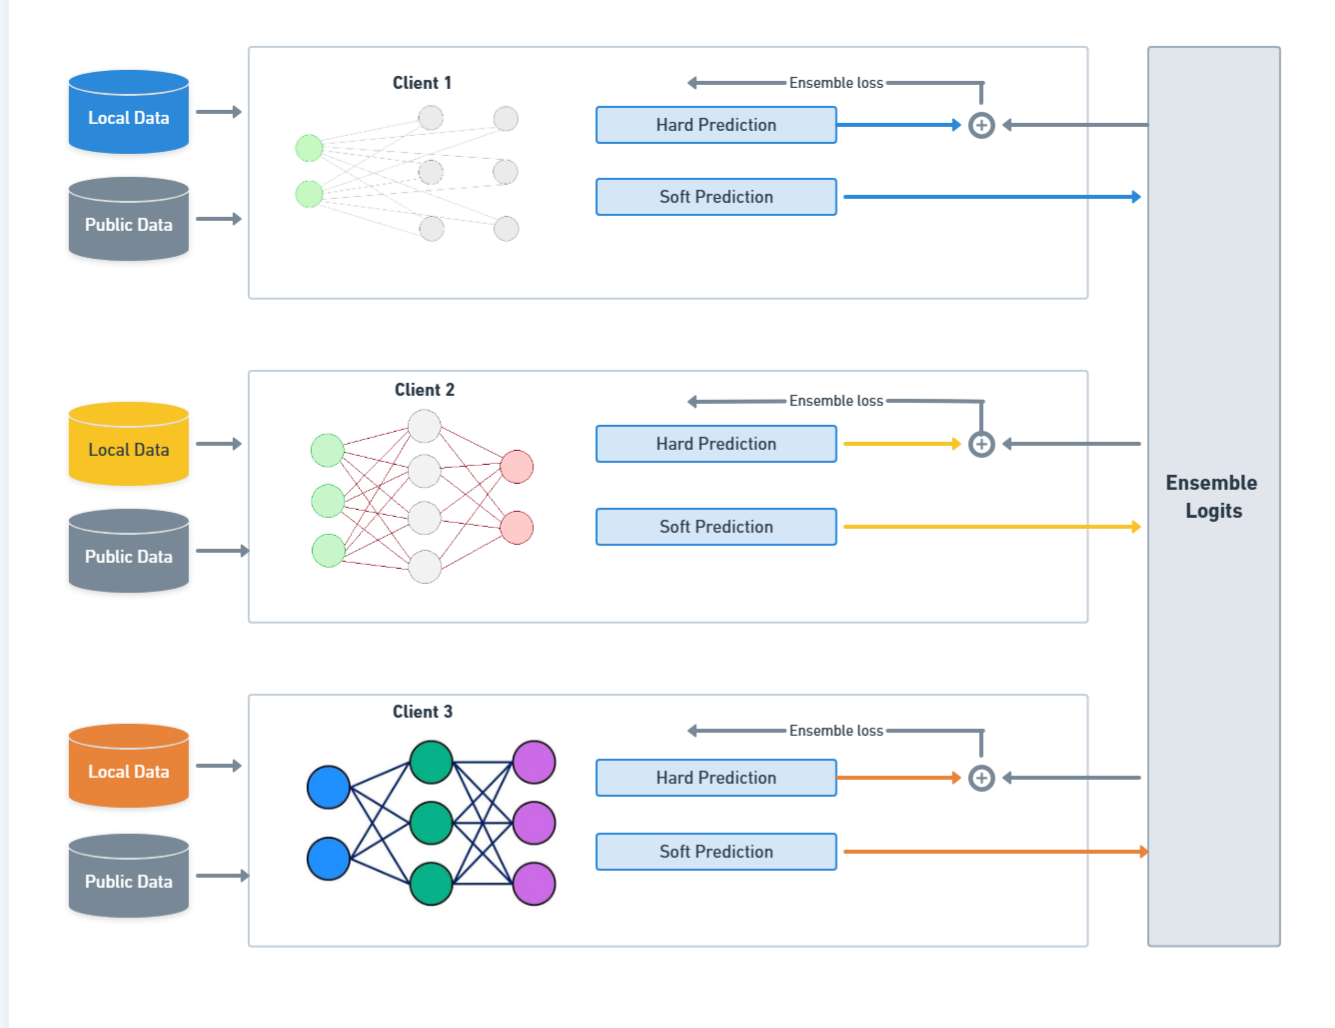
\includegraphics[width=0.75\linewidth]{Figures/KD.png}
%          \caption{Knowledge distillation}
%          \label{fig:enter-label}
%      \end{figure}

%     \begin{itemize}
        
%         \item Partial Training: Rather than training full models, devices may update only select layers, thereby lowering computational requirements while still contributing effectively to the global model. [arXiv:2312.12091v2]
        
%     \end{itemize}
%     \begin{figure}[H]
%         \centering
%         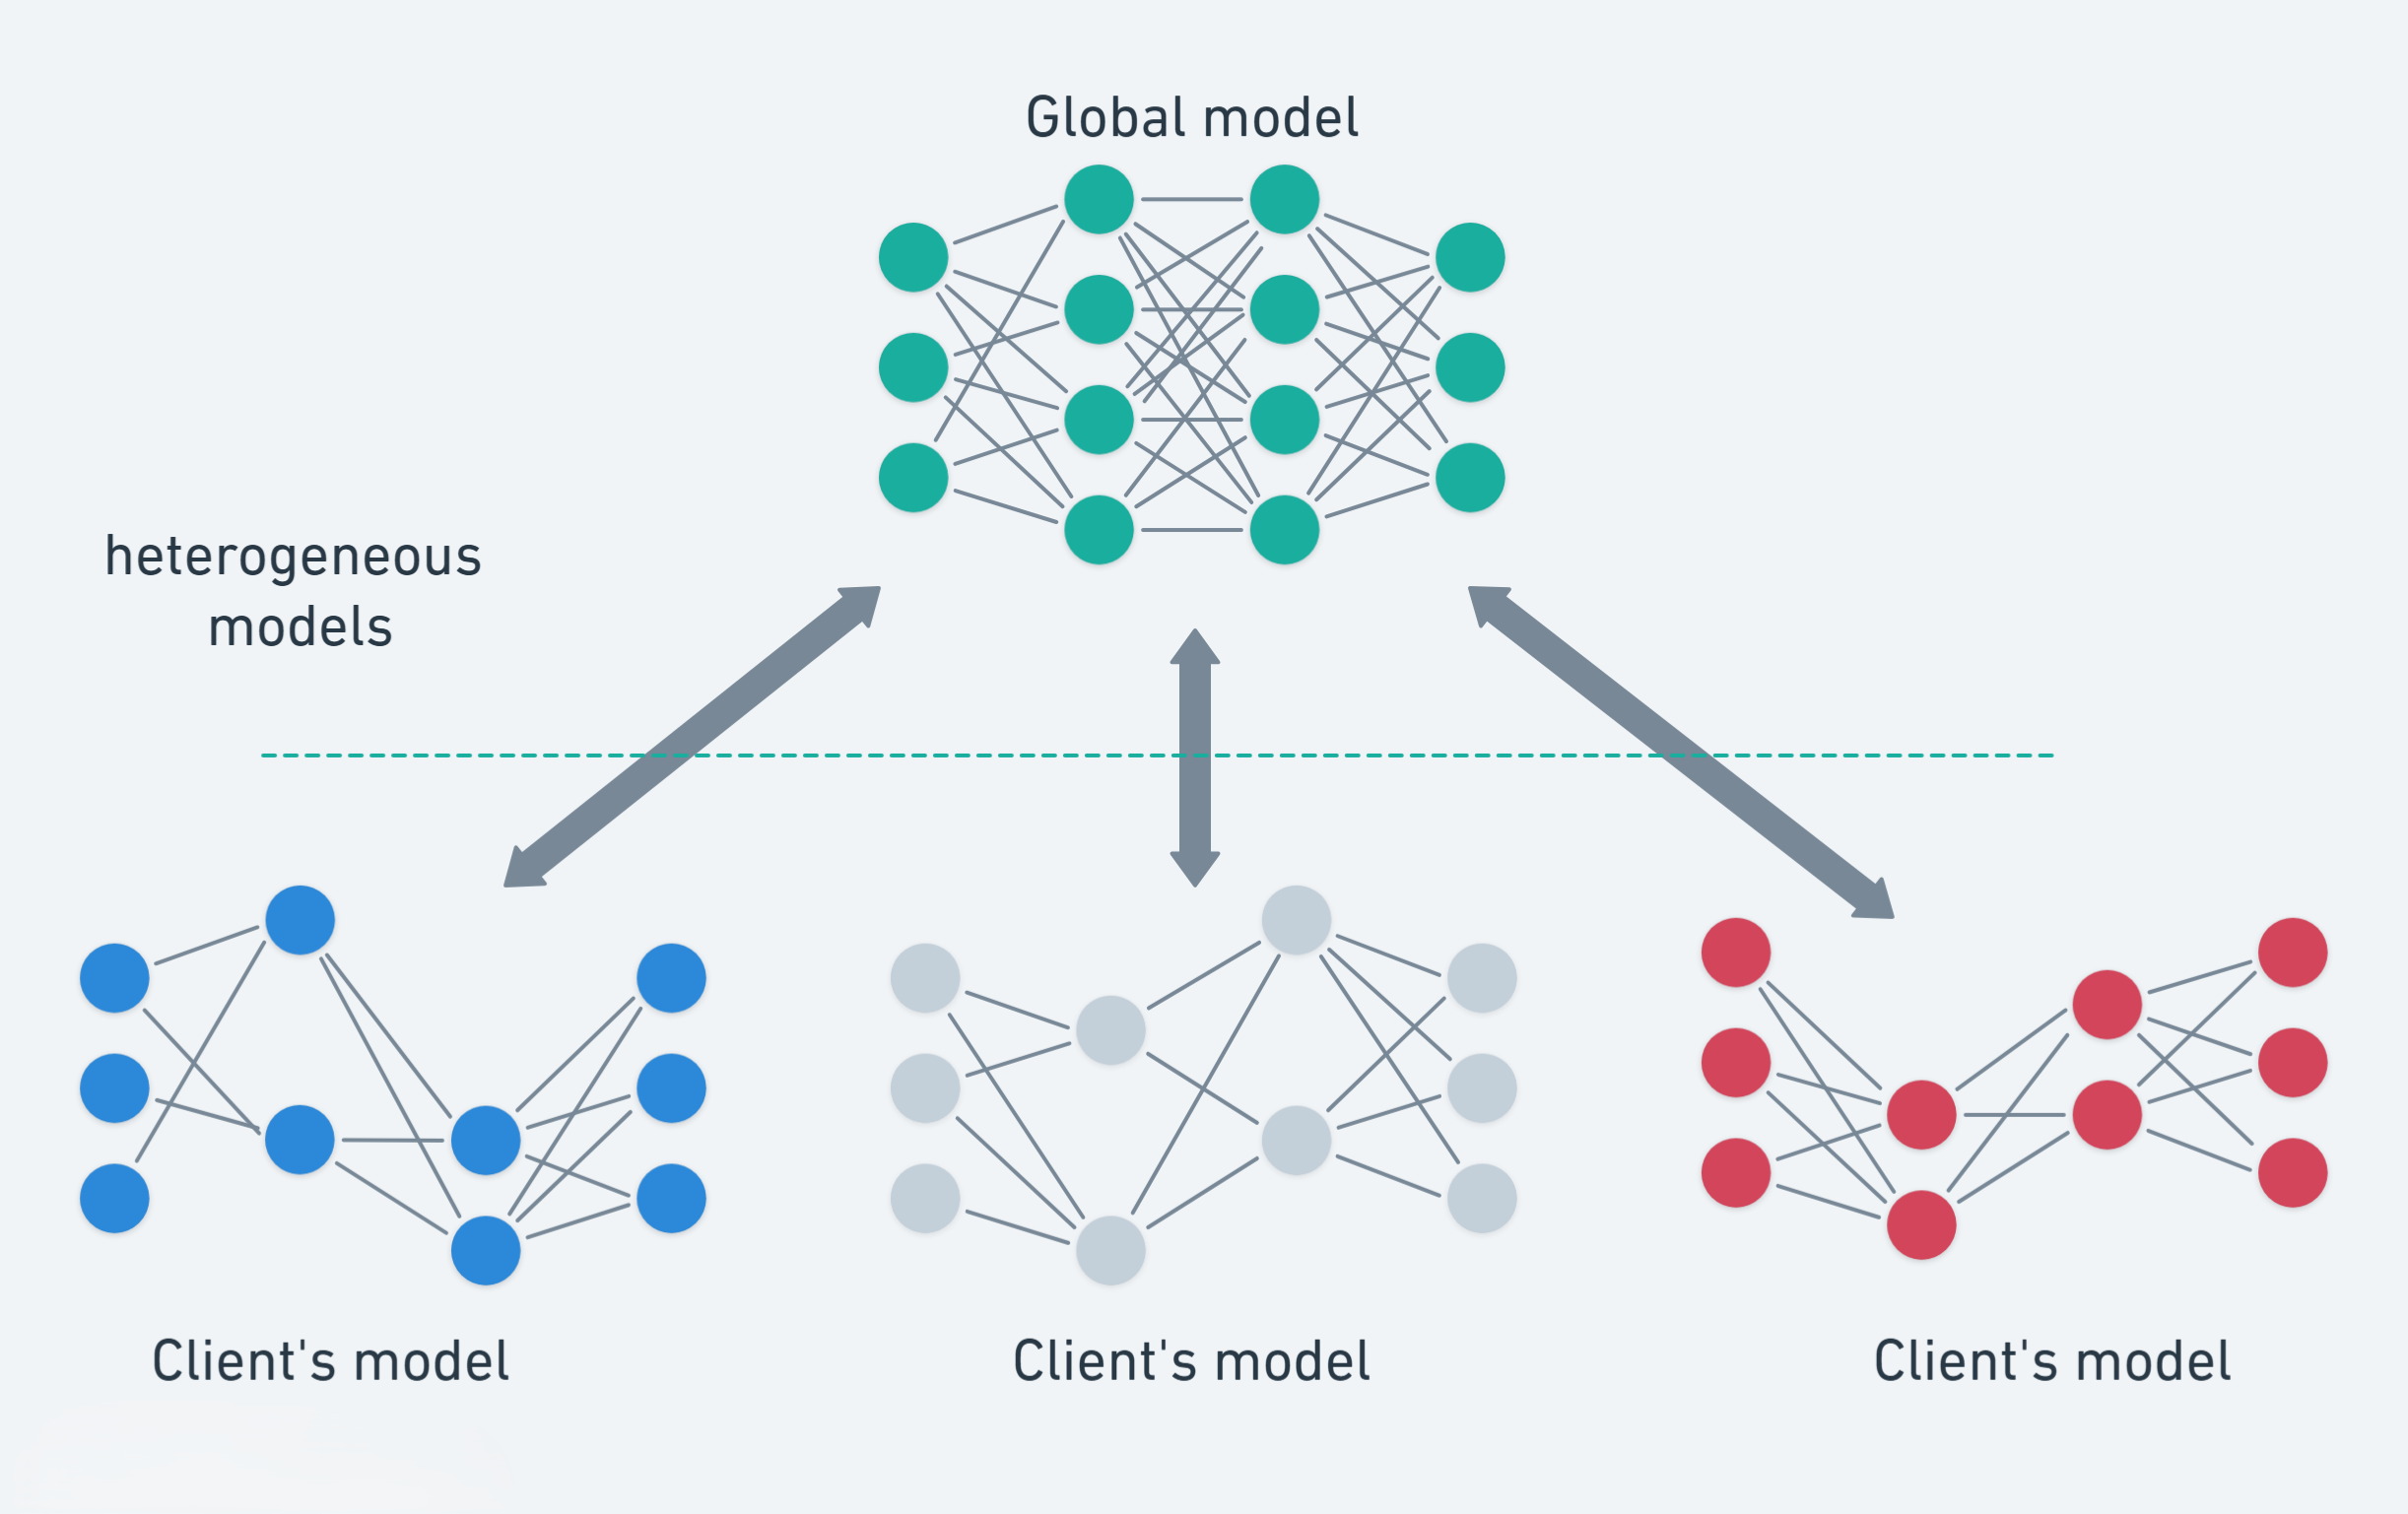
\includegraphics[width=0.5\linewidth]{Figures/partial_training.png}
%         \caption{partial training }
%         \label{fig:enter-label}
%     \end{figure}

%     \item Adaptive Aggregation: Enhancing Model Convergence
%     A persistent challenge in FL is the heterogeneity of data distributions (non-IID data) across devices, which can hinder model convergence. Recent advances include:

%     \begin{itemize}
%         \item \textbf{FedProx:} Incorporates a proximal term during local training to reduce the deviation from the global model, thereby stabilizing the training process.
%         \item \textbf{FedRolex:} A framework that enhances heterogeneous model training by using a rolling sub-model extraction method. It dynamically extracts and trains different sub-models over time, ensuring uniform training across the global model and mitigating client drift.
%         \item \textbf{SCAFFOLD:} Utilizes control variates to correct for client drift, thus mitigating the effect of local updates that might otherwise skew the global model.
%         \item \textbf{Dynamic Client Weighting:} Adjusts the contribution of each client's update according to data quality and size, ensuring that the aggregation process is balanced and robust.
%     \end{itemize}
% \end{itemize}

% These adaptive aggregation strategies have significantly improved FL performance and reliability in heterogeneous environments [2302.11466v2.pdf, arXiv:2312.12091v2].
\section{Types of Federated Learning}
\subsection{Based on Data Distribution}

\subsubsection{Horizontal Federated Learning (HFL)}
\begin{figure}[H]
    \centering
    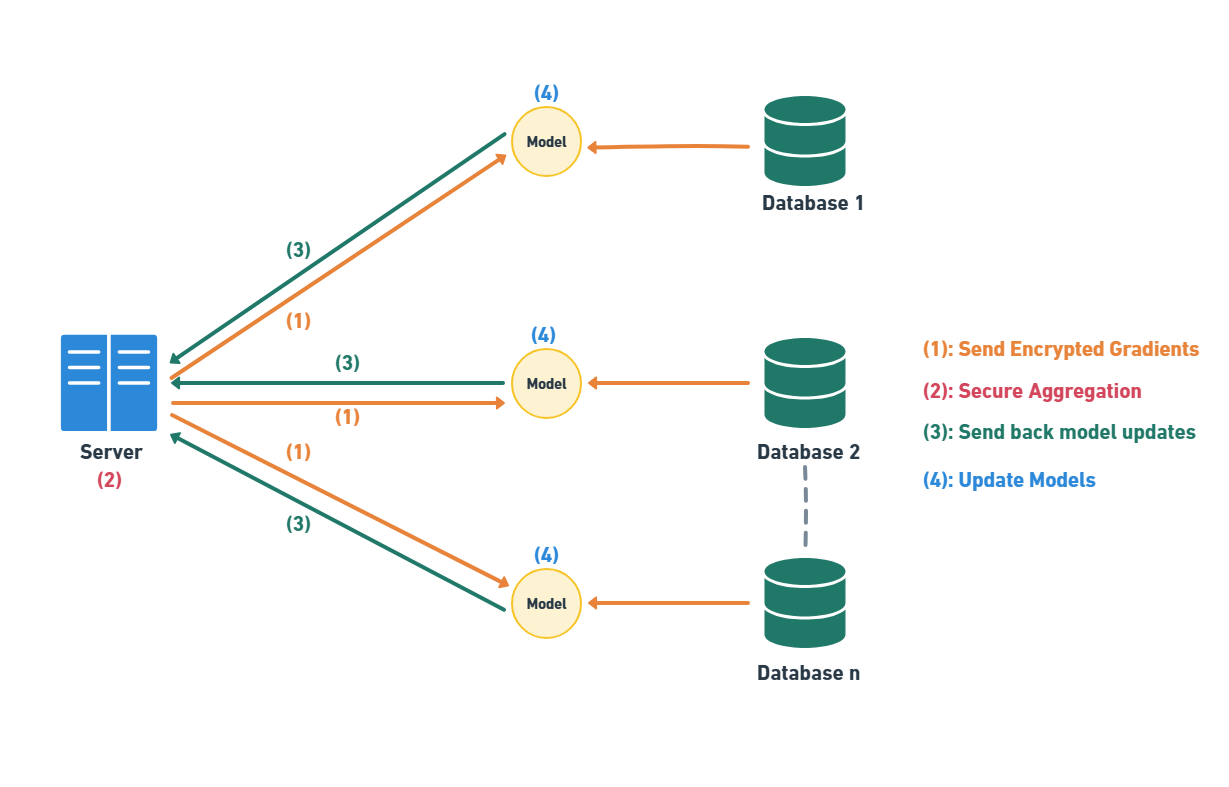
\includegraphics[width=0.75\linewidth]{Figures/diagram 1 (2).png}
    \caption{Horizontal Federated Learning}
    \label{fig:enter-label}
\end{figure}

Horizontal Federated Learning (HFL) is a decentralized machine learning approach in which multiple participants collaboratively train a shared global model without exchanging raw data. Each participant holds datasets with the same feature space, such as hospitals collecting identical health metrics, but with different data samples, ensuring both data privacy and compliance with protection regulations.




\subsubsection{Vertical Federated Learning (VFL)}
\begin{figure}[H]
    \centering
    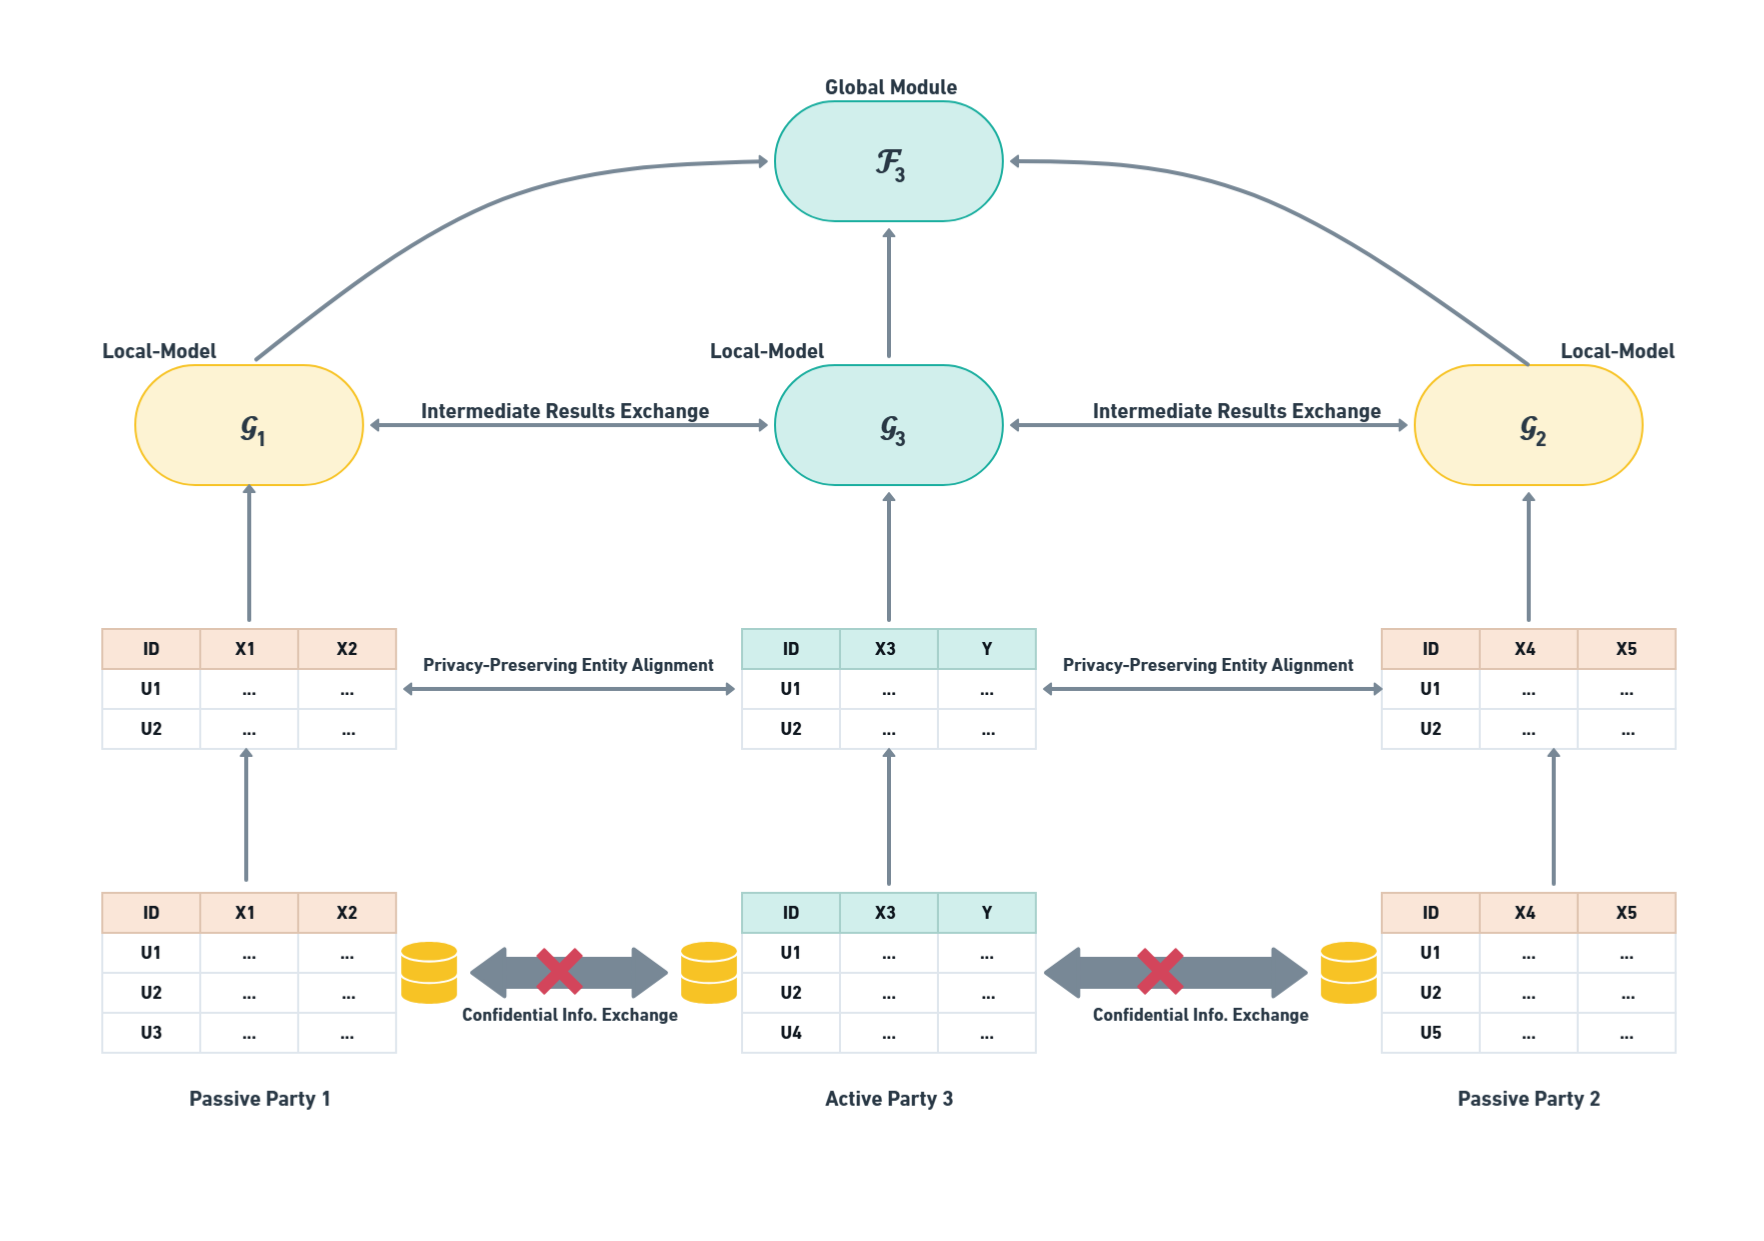
\includegraphics[width=0.75\linewidth]{Figures/VFL.png}
    \caption{Vertical Federated Learning}
    \label{fig:enter-label}
\end{figure}

Vertical Federated Learning (VFL) is tailored for scenarios where different organizations possess complementary features about the same individuals. For example, a bank can have access to a customer’s financial records, while a retailer holds their purchase history. By collaborating, these entities can train a more comprehensive model without revealing their raw data. In VFL, the feature space is partitioned, which means that each participant has a distinct subset of features for the same set of users,





\section{Based On Network Structure}

\begin{figure}[H]
    \centering
    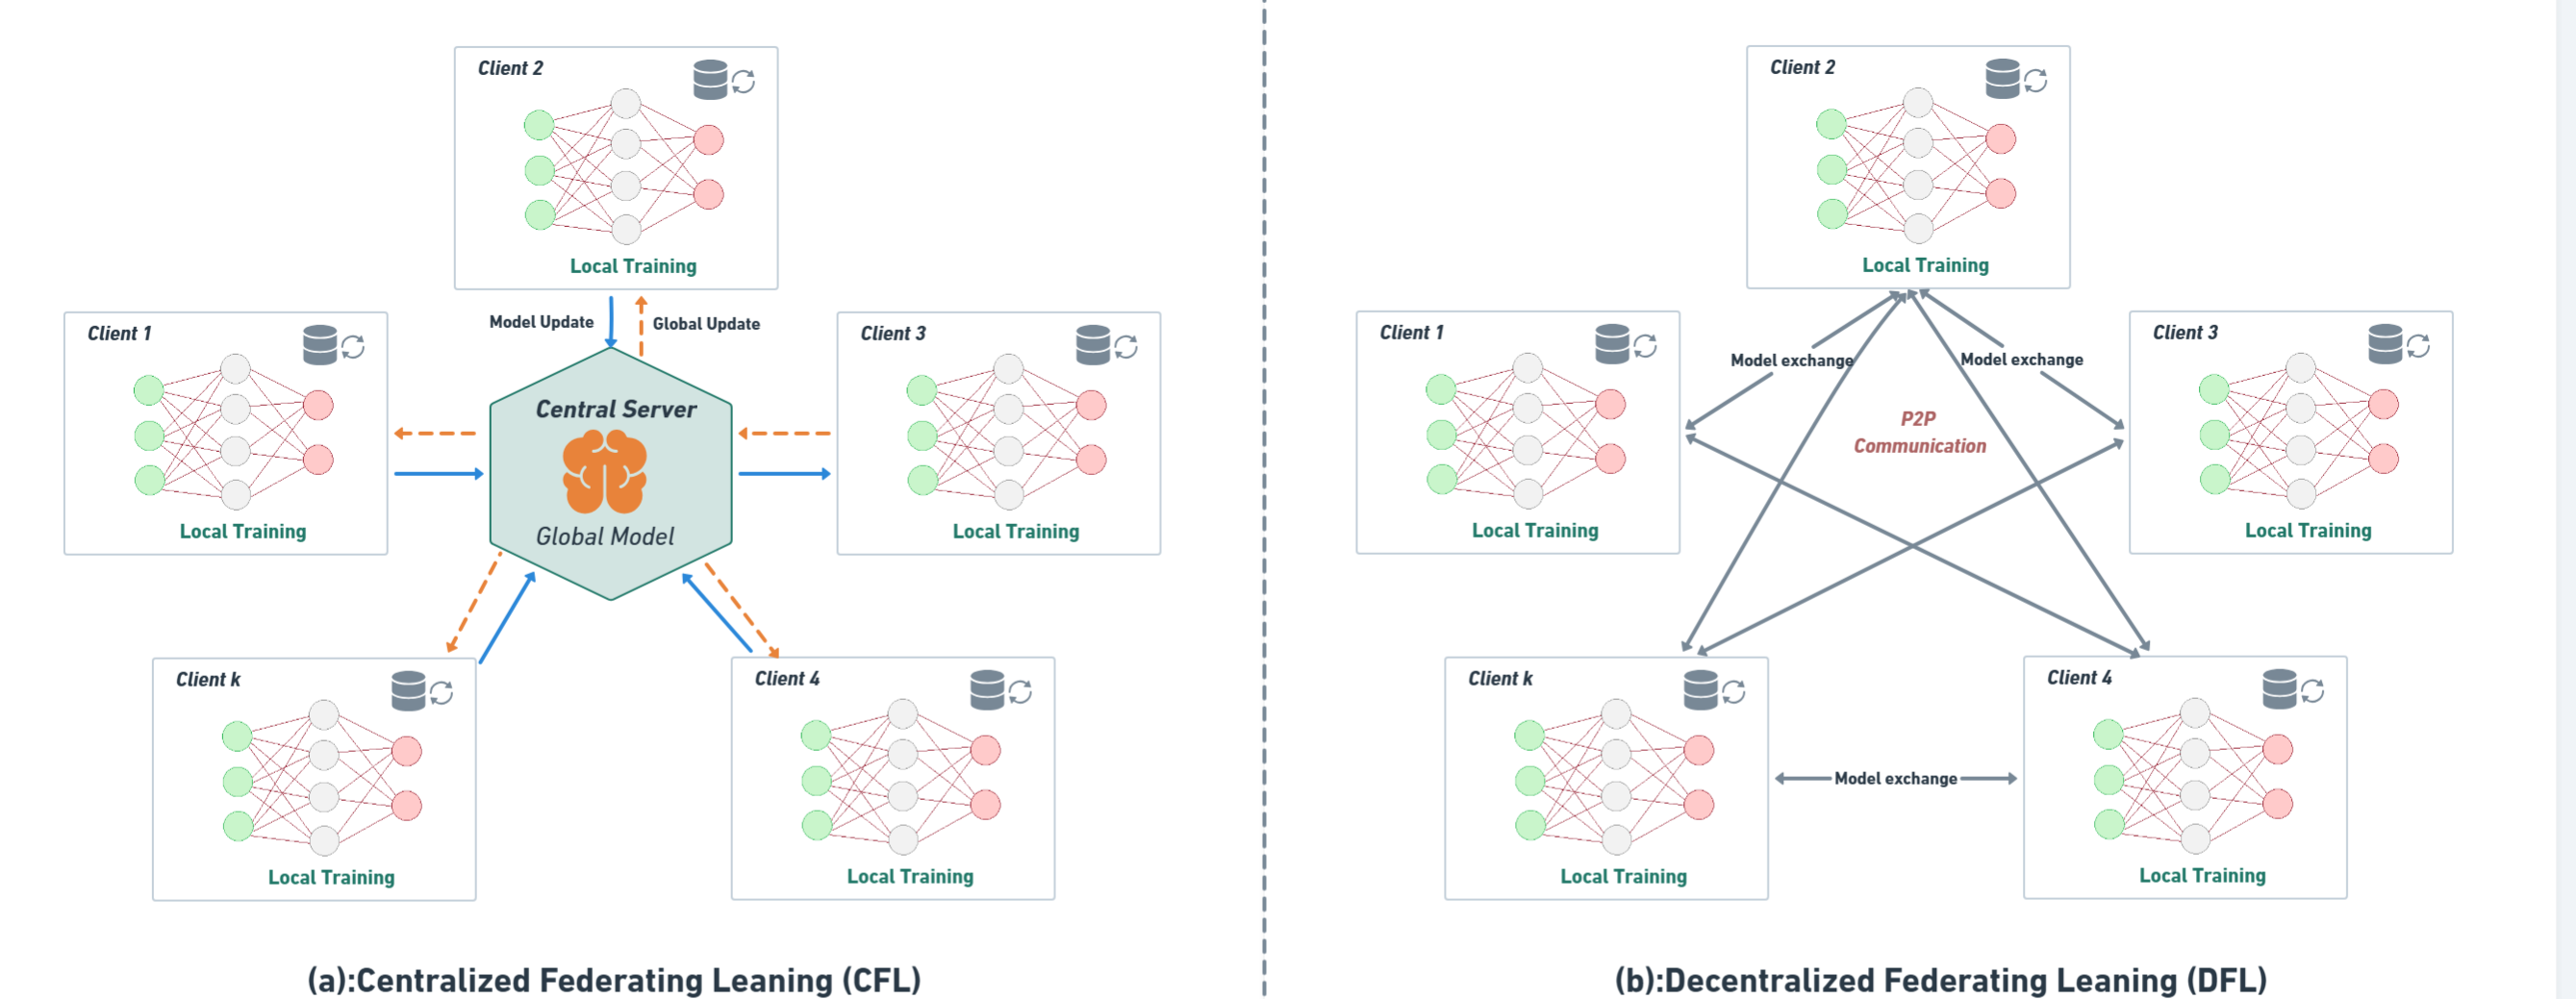
\includegraphics[width=1\linewidth]{Figures/network_based.png}
    \caption{Network Based Architecture}
    \label{fig:enter-label}
\end{figure}

Centralized Federated Learning (CFL) is a machine learning approach where a central server manages the coordination of training among multiple distributed clients. Each client trains a local model on its private data and periodically sends updates to the server. The server aggregates these updates to form a global model and redistributes it back to the clients. This setup allows data to remain local while still benefiting from collaborative learning across devices (Kairouz et al., 2021).

Decentralized Federated Learning (DFL) is a variation of federated learning that removes the need for a central server. Instead, clients communicate directly with each other in a peer-to-peer network to share model updates. Over time, these interactions lead to the development of a shared global model. DFL is particularly useful in environments where central coordination is not feasible or desired (Lalitha et al., 2019).




\section{Challenges and Solutions in Federated Learning}
\subsection{Privacy and Security Challenges}

Federated Learning (FL) faces significant challenges in maintaining data privacy and security during the collaborative training process. Since data remains on local devices, privacy-preserving techniques  such as encryption and differential privacy  are employed to prevent unauthorized access and ensure only aggregated model updates are shared [2].

Another major concern is the potential for malicious participants to inject biased or harmful updates into the training process. To mitigate this, secure aggregation protocols are implemented to verify the integrity and authenticity of model updates, ensuring the robustness of the final model.

 
% \subsubsection{Differential Privacy Techniques:}
% Differential privacy is a technique used to safeguard individual data privacy while permitting statistical analysis. In FL, differential privacy can be applied to add noise to the model updates before aggregation, avoiding the extraction of individual-level info.
% This practice helps to protect against membership inference attacks and statistical inference attacks on individual data [2].

\subsection{Communication and Resource Constraints}

Communication efficiency is crucial in FL, particularly when dealing with large-scale datasets or resource-constrained devices. To reduce communication overhead, techniques like model compression, quantization, and selective update transmission can be employed. These techniques reduce the amount of data transmitted between the local devices and the central server, which ultimately improves communication efficiency [2].
% \subsubsection{Bandwidth and Latency Constraints:}
% Bandwidth and latency constraints pose significant challenges in FL, mainly in scenarios with limited network resources. FL frameworks employ techniques such as gradient compression, adaptive communication scheduling, and bandwidth-efficient protocols to alleviate these constraints. These techniques aim to lessen the amount of data transmitted and optimize the communication schedule, reducing the impact of bandwidth and latency limitations.
% Adaptive Communication and Model Compression Techniques:
% Adaptive communication techniques automatically regulate the communication frequency or data exchanged based on the relevance of the local data. This allows more efficient utilization of network resources. Moreover, model compression techniques, such as knowledge distillation and pruning, can reduce the size of the model, supporting faster and more effective communication between the local devices and the central server [2].

\subsection{Heterogeneity and Data Distribution}
Data and Model Heterogeneity Handling Strategies:
FL frameworks need to deal with heterogeneity in terms of data types, formats, and model architectures among various participating devices. Techniques such as transfer learning meta-learning, and model aggregation with model selection can be used to handle heterogeneity. These approaches permit the central server to adjust and combine models trained on different types of data or models with varying architectures [2].
Federated Transfer Learning and Meta-Learning Approaches:
Federated Transfer Learning facilitates the transfer of knowledge from a pre-trained global model to local models, which helps increase learning productivity and performance [2].

% \subsection{Real-World Applications }
% While Federated Learning (FL) has been extensively explored in fields such as healthcare and finance, its application in environmental monitoring, particularly in water quality assessment, remains an emerging area of research. Recent studies have begun investigating its potential to enable privacy-preserving, real-time analysis of sensor data while addressing key challenges such as data heterogeneity and communication constraints. Existing projects leverage FL to enhance data privacy, computational efficiency, and scalability, particularly in real-time anomaly detection for water systems.
% One notable study introduces the MCN-LSTM (Multivariate Convolutional Neural Network with Long Short-Term Memory) approach for anomaly detection in water quality monitoring. This method integrates deep learning techniques to process and analyze large volumes of time-series data collected from IoT-enabled sensors. Unlike traditional centralized machine learning models, which require transferring raw environmental data to a central server, FL allows models to be trained locally on sensor nodes before aggregating updates in a decentralized manner, thereby improving data security and reducing bandwidth consumption.
% Several projects have explored FL for water quality prediction. For example, Wu et al. (2022) applied FL with LSTMs to monitor river water quality, achieving an RMSE of 0.12 pH units. Similarly, Zhang et al. (2023) used federated CNNs for detecting algal blooms from satellite imagery, demonstrating FL’s capability to process spatially distributed data while preserving data locality. Additionally, FL-based pollution tracking has been enhanced using anomaly detection methods such as Isolation Forest, which processes real-time data streams from distributed air and water sensors to identify sudden pollution spikes.
% Despite these advancements, FL-based approaches for water quality monitoring still 
% face significant technical barriers. Data heterogeneity remains a major challenge due to seasonal variations and the diversity of sensor types (e.g., pH probes vs. turbidity sensors), which can affect the consistency of model updates across decentralized nodes. Moreover, regulatory constraints, such as GDPR compliance, complicate cross-border data sharing in international water systems. These challenges highlight the need for more adaptive FL frameworks capable of operating across diverse environments while ensuring robust privacy, security, and computational efficiency.[3]

\newpage

\section*{Conclusion}


This chapter reviewed the current advancements in Federated Learning (FL), tracing its development from foundational concepts to recent innovations addressing scale and diversity. It covered various FL types based on data and network structures, showcasing FL's adaptability. While FL offers significant advantages, especially in privacy, it still faces challenges like security, communication overhead, and data heterogeneity, which are active research areas. The chapter also noted FL's emerging application in environmental monitoring, such as water quality, underscoring FL's growing importance for private, distributed data analysis.


























